\documentclass[3p]{elsarticle} %preprint/3p

\usepackage{hyperref}

\journal{ }

\usepackage{amsmath} %added for maths environments (equation and align)
\usepackage{amssymb}
\usepackage{bm} %bold symbols by using \bm
\usepackage{mathtools} %added for \xrightleftharpoons

\usepackage{subcaption} %allowing for subcaptions and subfigures
\captionsetup[sub]{font=normalsize}%normalsize

\usepackage[autostyle]{csquotes}
\MakeOuterQuote{"}

% slightly altering rules for figure placement to prevent full-page figures
\usepackage{placeins}
\renewcommand{\floatpagefraction}{.90}
\renewcommand{\topfraction}{.90}

\usepackage[capitalise]{cleveref}

\usepackage{todonotes} %added for todo notes
\let\oldtodo\todo
\renewcommand{\todo}[1]{\oldtodo[inline]{#1}}
%\renewcommand{\todo}[1]{\oldtodo[color=white!40,inline]{#1}}
\newcommand{\toask}[1]{\oldtodo[color=green!40, inline]{#1}}
\newcommand{\wrn}[1]{\oldtodo[color=red!40, inline]{#1}}

\usepackage{xcolor}
\usepackage{listings}
\usepackage{lstautogobble}
\usepackage[numbered]{matlab-prettifier}
\lstdefinestyle{mystyle}{
	numbers=left,
	numberstyle=\footnotesize,
	numbersep=8pt,
	style=Matlab-editor,
	tabsize=4,
	basicstyle=\ttfamily\footnotesize,
	numbersep=25pt,
	frame=none,
	autogobble=true
}

\newcommand{\citeMe}{\href{http://www.doi.org/10.1149/1945-7111/acb971}{T. Hageman \& E. Martínez-Pañeda, \textit{Stabilising effects of lumped integration schemes for the simulation of metal-electrolyte reactions}. Journal of The Electrochemical Society (2023)}}

\begin{document}

\begin{frontmatter}
\title{Lumped Electrochemistry: a MATLAB code to utilize the stabilising effects of lumped integration schemes for the simulation of metal-electrolyte reactions}

\author{Tim Hageman \corref{mycorrespondingauthor}}
\cortext[mycorrespondingauthor]{Corresponding author}
\ead{t.hageman@imperial.ac.uk}
\author{Emilio Martínez-Pañeda}

\address{Department of Civil and Environmental Engineering, Imperial College London, London SW7 2AZ, UK}

\begin{abstract}
Documentation that accompanies the \textit{MATLAB} code lumped electrochemistry. This documentation explains the usage of the implemented finite element framework, and highlight the main files. Special attention is paid to the parts of the code that implement the volume and interface reactions, which are integrated using a lumped integration scheme. 

If using this module for research or industrial purposes, please cite: \citeMe{}.
\end{abstract}

\begin{keyword}
MATLAB, electrochemistry, finite element method, lumped integration, oscillations, hydrogen absorption
\end{keyword}

\end{frontmatter}

\tableofcontents

\section{Introduction}
\begin{figure}
    \centering
    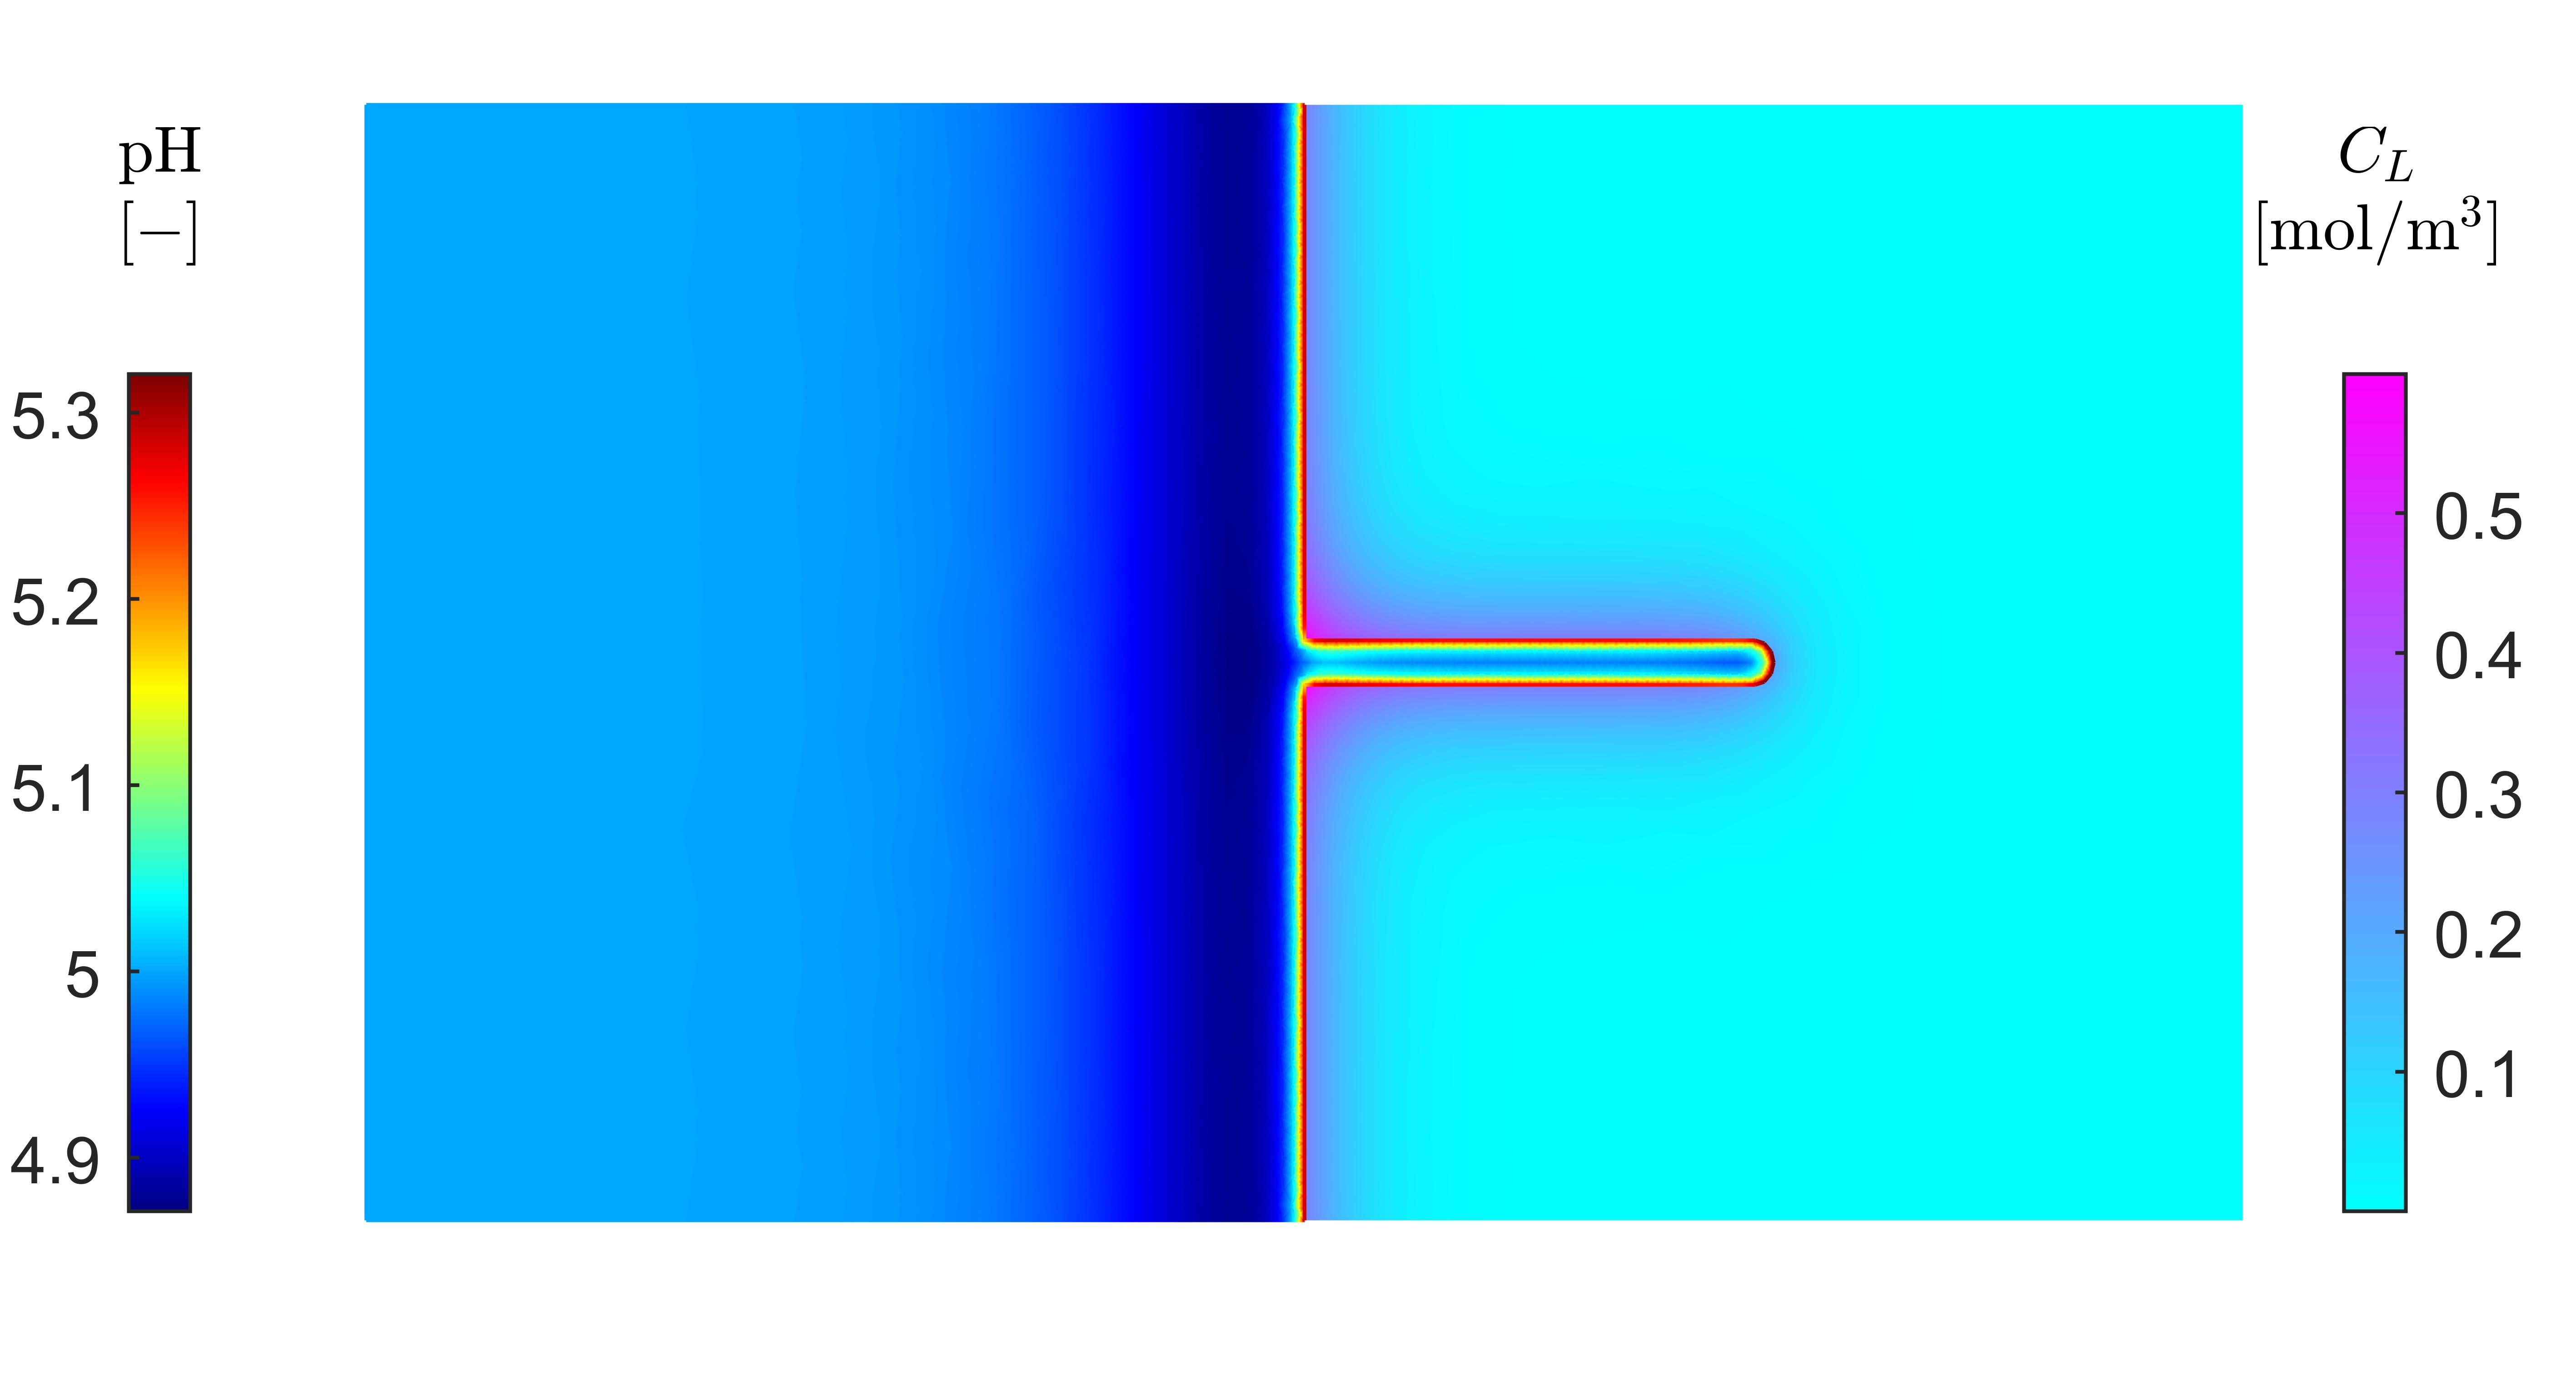
\includegraphics[width=12cm]{../Figures/SurfacePlot.jpg}
    \caption{Example of surface data plotted during the post-processing procedure.}
    \label{fig:example_surf}
\end{figure}

Electro-chemical systems often include reactions with rates varying by several orders of magnitude. Some reaction rates might enforce a near-instant equilibrium, while others occur over many hours to years. While it is possible to enforce equilibrium reactions a priori, this requires assumptions of the dominant reaction mechanics which limit the applicability of the resulting model to a narrow range of circumstances. In contrast, when chemical reactions are modelled as-is, the numerical models are commonly hindered by poor convergence rates or spurious oscillations, both of which require small time increments and which make simulating realistic time-scales costly or even infeasible. Here, the numerical model, implemented within MATLAB, is presented that accompanies \citeMe{}. This model uses a lumped integration scheme, which has been shown to greatly improve the stability. The remainder of this documentation first discusses basic usage of the provided finite element method code, then provides a more in-depth description of the implementation aspects and components of the code, and finally discusses the lumped integration scheme in detail. This code has been verified to work with matlab versions 2021b and 2022a, older versions might not be compatible. 

DISCLAIMER: While this code has been cross-verified with comparison to simulation results from the commercial finite element package COMSOL, it can not be guaranteed to be error-free. Before using this code for relevant or critical applications, especially when simulating cases not directly included, please perform your own verification. The authors are not responsible for any issues arising from mistakes within this matlab code.

\subsection{Basic usage}
For simulating the model as provided, running the function "main.m" performs all required actions: It automatically generates the geometry and mesh, initialises all simulation components, and prints outputs to the screen and saves them to a folder within results. Simple changes, e.g. editing parameters, can be done within main.m without requiring altering other files. A separate file is present to perform post-processing based on saved output files, "PostProcessing.m", which based on a path to the output files visualises the results.

\section{Summary of included files}
The code is set up in a object-oriented manner, defining matlab classes for each sub-component and providing their accompanying methods. As a result, a clear distinction is made between different components, and each can be used and altered with limited/no impact on other components. Here, the different classes are described. The commenting style employed within the code is compatible with the matlab help function, as such information about all usable methods within a class can be accessed by including the relevant folders, and typing, for instance, "help Solver" to print all variables contained within and all function available from the solver. 

\subsection{main.m}
This is the main file, from which all classes are constructed and the actual simulation is performed. Within it, all properties used within other classes are defined as inputs, for instance for the linear-elastic description of the solid domain:
\lstinputlisting[firstnumber=59,firstline=59,lastline=63,style=mystyle,title=main.m]{../main.m}
where "physics{\_}in" is the array of options (in this case, physical models) passed to the physics object at construction. 

The actual time-dependent simulations are also performed within this file:
\lstinputlisting[firstnumber=164,firstline=164,lastline=171,style=mystyle,title=main.m]{../main.m}
\lstinputlisting[firstnumber=191,firstline=191,lastline=194,style=mystyle]{../main.m}
Notably, while this performs the time-stepping scheme and controls the time increment size and termination of the simulations, it does not by itself solve anything, instead calling the "solver.Solve()" function which performs a Newton-Raphson procedure using the parameters used to initialize the class, and once the current timestep is converged returns to the main code.

\subsection{Models}
The files included within the Models folder form the main implementation of all the physical phenomena involved. They implement the assembly of tangential matrices and force vectors, when requested by the solving procedures, and store model-specific parameters. 

\subsubsection{BaseModel}
This is an empty model, inherited by all other models to provide consistency within the available functions. While empty within here, the potential functions that can be defined within other models include assembling the system matrix and force vector:
\lstinputlisting[firstnumber=26,firstline=26,lastline=26,style=mystyle,title=Models/@BaseModel/BaseModel.m]{../Models/@BaseModel/BaseModel.m}
, and committing history dependent or path dependent variables:
\lstinputlisting[firstnumber=13,firstline=13,lastline=13,style=mystyle]{../Models/@BaseModel/BaseModel.m}
where the keyword "commit{\_}type" indicates the type of history or path dependence to commit at the current point. 

\subsubsection{Constrainer}
This model is used to apply fixed boundary constraints to a degree of freedom at a set location. Within the main file, the inputs required are:
\lstinputlisting[firstnumber=72,firstline=72,lastline=75,style=mystyle,title=main.m]{../main.m}
and multiple definitions of this model are allowed, allowing for constraints to be applied to several element groups. These constraints are integrated within the tangential matrix and force vector through  allocation matrices $\bm{C}_{con}$ and $\bm{C}_{uncon}$, reordering the system into a constrained and unconstrained part. This allows the constrained system to be solved as:
\begin{equation}
	\bm{C}_{uncon}^T \bm{K} \bm{C}_{uncon} \mathbf{y} = -\left(\bm{C}_{uncon}^T\bm{f}+\bm{C}_{uncon}^T \bm{K} \bm{C}_{con}\mathbf{c}\right)
\end{equation}
with the values of the boundary constraints contained in the vector $\mathbf{c}$. After solving, the state vector is then incremented through:
\begin{equation}
	\mathbf{x}^{new} = \mathbf{x}^{old} + \bm{C}_{uncon}\mathbf{y} + \bm{C}_{con}\mathbf{c}
\end{equation}


\subsubsection{LinearElastic}
The linear-elastic model implements the momentum balance for the metal domain:
\begin{equation}
	\bm{\nabla}\cdot\bm{\sigma} = \mathbf{0}
\end{equation}
where the stresses $\bm{\sigma}$ are based on the displacement $\mathbf{u}=["\mathrm{dx}"\;"\mathrm{dy}"]$. The properties used to initialize this model given as input by:
\lstinputlisting[firstnumber=59,firstline=59,lastline=63,style=mystyle,title=main.m]{../main.m}
Notably, since the tangential matrix for linear-elasticity is constant, it is assembled once and saved locally within the model, after which during the global matrix assembly process, it is copied over to the global matrix:
\lstinputlisting[firstnumber=103,firstline=103,lastline=105,style=mystyle,title=Models/@LinearElastic/LinearElastic.m]{../Models/@LinearElastic/LinearElastic.m}
with the force vector also being updated based on this locally saved stiffness matrix. 

\subsubsection{HydrogenDiffusion}
This model implements the hydrogen mass conservation, through the diffusion equation:
\begin{equation}
    \dot{C}_L + \bm{\nabla}\cdot\left(-\frac{D_L}{1-C_L/N_L} \bm{\nabla}C_L \right) + \bm{\nabla}\cdot\left(\frac{D_L C_L \overline{V}_H}{RT}\bm{\nabla}\sigma_H\right) = 0
\end{equation}
with the interstitial lattice hydrogen concentration $C_L$ indicated within the code by "CL". Input properties for this model constitute:
\lstinputlisting[firstnumber=65,firstline=65,lastline=69,style=mystyle,title=main.m]{../main.m}
This model presumes the linear-elastic model is provided within input 1, from which the Young's modulus and Poisson ratio are taken.

\subsubsection{Electrolyte}
The electrolyte model implements the Nernst-Planck mass balance:
\begin{equation}
    \dot{C}_{\pi}+\bm{\nabla}\cdot\left(-D_\pi \bm{\nabla}C_\pi\right) + \frac{z_\pi F}{RT} \bm{\nabla} \cdot \left(-D_\pi C_\pi \bm{\nabla} \varphi\right) +R_\pi = 0 
\end{equation}
for the ionic species and their name within the model file: $\mathrm{H}^+$ ("H"), $\mathrm{OH}^-$ ("OH"), $\mathrm{Na}^+$ ("Na"), $\mathrm{Cl}^-$ ("Cl", using lower case l; upper case L provides the lattice hydrogen concentration), $\mathrm{Fe}^{2+}$ ("Fe"), and $\mathrm{FeOH}^{+}$ ("FeOH"). Additionally, it implements the electro-neutrality condition:
\begin{equation}
	\sum z_\pi C_\pi = 0
\end{equation}
and bulk reactions:
\begin{equation}
    \mathrm{H}_2\mathrm{O} \xrightleftharpoons[k_{w}']{k_{w}} \mathrm{H}^+ + \mathrm{OH}^- \label{react:water}
\end{equation}
\begin{equation}
    \mathrm{Fe}^{2+} + \mathrm{H}_2\mathrm{O} \xrightleftharpoons[k_{fe}']{k_{fe}} \mathrm{FeOH}^+ + \mathrm{H}^+ \label{react:fe_feoh}
\end{equation}
\begin{equation}
    \mathrm{FeOH}^{+} + \mathrm{H}_2\mathrm{O} \xrightharpoonup{k_{feoh}} \mathrm{Fe}(\mathrm{OH})_2 + \mathrm{H}^+ \label{react:feoh_feoh2}
\end{equation}
with reaction rates:
\begin{equation}
    R_{\mathrm{H}^+,w}=R_{\mathrm{OH}^-} = k_{w}C_{\mathrm{H}_2\mathrm{O}} - k_{w}'C_{\mathrm{H}^+}C_{\mathrm{OH}^-}  = k_{eq} \left(K_w-C_{\mathrm{H}^+} C_{\mathrm{OH}^-} \right) \label{eq:water_react}
\end{equation}
\begin{align}
    R_{\mathrm{Fe}^{2+}}&=-k_{fe}C_{\mathrm{Fe}^{2+}}+k_{fe}'C_{\mathrm{FeOH}^+}C_{\mathrm{H}^+} \\
    R_{\mathrm{FeOH}^+}&=k_{fe}C_{Fe^{2+}}-C_{\mathrm{FeOH}^+}(k_{feoh}+k_{fe}'C_{\mathrm{H}^+})\\
    R_{\mathrm{H}^+,fe}&=k_{fe}C_{\mathrm{Fe}^{2+}}-C_{\mathrm{FeOH}^+}(k_{fe}'C_{\mathrm{H}^+}-k_{feoh}) \label{eq:H_Part2}
\end{align}
For this model, the input properties required are:
\lstinputlisting[firstnumber=92,firstline=92,lastline=100,style=mystyle,title=main.m]{../main.m}
This model employs a lumped integration scheme when the vector "Lumped" contains true. Details for the implementation of this lumped scheme are given in \cref{sec:LumpedScheme}

\subsubsection{ElectrolyteInterface}
Finally, the electrolyteInterface model implements the metal-electrolyte coupling through the surface reactions:
\begin{alignat}{2}
 \text{Volmer (acid):} && \mathrm{H}^+ + \mathrm{M} + \mathrm{e}^- &\xrightleftharpoons[k_{Va}']{k_{Va}} \mathrm{MH}_{ads} \label{react:1} \\
  \text{Heyrovsky (acid):} && \qquad \mathrm{H}^+ + \mathrm{e}^- + \mathrm{MH}_{ads}&\xrightleftharpoons[k_{Ha}']{k_{Ha}} \mathrm{M} + \mathrm{H}_2 \label{react:2} \\
    \text{Volmer (base):} &&  \mathrm{H}_2\mathrm{O} + \mathrm{M} + \mathrm{e}^- &\xrightleftharpoons[k_{Vb}']{k_{Vb}} \mathrm{MH}_{ads} + \mathrm{OH}^- \label{react:5} \\
   \text{Heyrovsky (base):} && \qquad  \mathrm{H}_2\mathrm{O} + \mathrm{e}^- + \mathrm{MH}_{ads}&\xrightleftharpoons[k_{Hb}']{k_{Hb}} \mathrm{M} + \mathrm{H}_2 + \mathrm{OH}^- \label{react:6} \\
    \text{Tafel:} && 2 \mathrm{MH}_{ads} &\xrightleftharpoons[k_T']{k_T} 2\mathrm{M} + \mathrm{H}_2 \label{react:3} \\
   \text{Absorption:} && \mathrm{MH}_{ads} &\xrightleftharpoons[k_A']{k_A} \mathrm{MH}_{abs}  \label{react:4} \\
   \text{Corrosion:} && \qquad  \mathrm{Fe}^{2+}+2\mathrm{e}^- &\xrightleftharpoons[k_c']{k_c} \mathrm{Fe} \label{react:7}
\end{alignat}
with reaction rates:
\begin{alignat}{4}
\nonumber && && & \qquad\mathrm{Forward} &&  \qquad\qquad \mathrm{Backward} \\
    \mathrm{Volmer (acid):} && \quad && \nu_{Va} &= k_{Va} C_{\mathrm{H}^+}(1-\theta_{ads})e^{-\alpha_{Va} \frac{\eta F}{RT}}\qquad
    && \nu_{Va}' = k_{Va}' \theta_{ads}e^{(1-\alpha_{Va}) \frac{\eta F}{RT}} \label{eq:react1}\\
    \mathrm{Heyrovsky (acid):} && && \nu_{Ha} &= k_{Ha} C_{\mathrm{H}^+}\theta_{ads}e^{-\alpha_{Ha} \frac{\eta F}{RT}}\qquad
    && \nu_{Ha}' = k_{Ha}' (1-\theta_{ads}) p_{\mathrm{H}_2} e^{(1-\alpha_{Ha}) \frac{\eta F}{RT}} \label{eq:react2}\\
    \mathrm{Volmer (base):} && && \nu_{Vb} &= k_{Vb} (1-\theta_{ads})e^{-\alpha_{Vb} \frac{\eta F}{RT}}\qquad
    && \nu_{Vb}' = k_{Vb}' C_{\mathrm{OH}^-} \theta_{ads}e^{(1-\alpha_{Vb}) \frac{\eta F}{RT}} \label{eq:react5}\\
    \mathrm{Heyrovsky (base):} && && \nu_{Hb} &= k_{Hb} \theta_{ads}e^{-\alpha_{Hb} \frac{\eta F}{RT}}\qquad
    && \nu_{Hb}' = k_{Hb}' (1-\theta_{ads}) p_{\mathrm{H}_2} C_{\mathrm{OH}^-} e^{(1-\alpha_{Hb}) \frac{\eta F}{RT}}  \label{eq:react6}\\
    \mathrm{Tafel:} && && \nu_T &= k_T\left|\theta_{ads}\right|\theta_{ads}\qquad
    && \nu_T' = k_T' (1-\theta_{ads})p_{\mathrm{H}_2} \label{eq:react3}\\
    \mathrm{Absorption:} && && \nu_A &= k_A (N_L - C_L)\theta_{ads}\qquad
    && \nu_A' = k_A' C_L (1-\theta_{ads}) \label{eq:react4}\\
    \mathrm{Corrosion:} && && \nu_{c} &= k_{c} C_{\mathrm{Fe}^{2+}}e^{-\alpha_{c} \frac{\eta F}{RT}} \qquad && \nu_{c}' = k_{c}' e^{(1-\alpha_{c}) \frac{\eta F}{RT}}   \label{eq:react7}
\end{alignat}
These reaction rates are implemented in a separate function from the matrix assembly:
\lstinputlisting[firstnumber=364,firstline=364,lastline=364,style=mystyle,title=Models/@ElectrolyteInterface/ElectrolyteInterface.m]{../Models/@ElectrolyteInterface/ElectrolyteInterface.m}
which takes the local hydrogen, hydroxide, and iron concentrations, the surface coverage, electrolyte potential, and interstitial lattice hydrogen concentration. It functions for both the integration-point variables as well as for the nodal values. These reaction rates are integrated through a lumped scheme, with details about this scheme discussed in \cref{sec:LumpedScheme}. In addition to the reaction rates, the electrolyte interface model also resolves the surface mass balance:
\begin{equation}
    N_{ads} \dot{\theta}_{ads} - (\nu_{Va}-\nu_{Va}') + \nu_{Ha} + 2 \nu_T + (\nu_A-\nu_A') - (\nu_{Vb}-\nu_{Vb}') + \nu_{Hb} = 0
\end{equation}
For this model, the input variables to define are given as:
\lstinputlisting[firstnumber=113,firstline=113,lastline=120,style=mystyle,title=main.m]{../main.m}
with the vector "Lumped" allowing for individual interface reactions to be either integrated using a standard Gauss integration scheme (0) or a lumped integration scheme (1). the reaction constants matrix k is defined as:
\begin{equation}
	k = \begin{bmatrix} 
	k_{Va} & k_{Va}' & \alpha_{Va} & E_{eq,Va} \\ 
	k_{Ha} & k_{Ha}' & \alpha_{Ha} & E_{eq,Ha} \\ 
	k_{T} & k_{T}' & - & - \\ 
	k_{A} & k_{A}' & - & - \\ 
	k_{Vb} & k_{Vb}' & \alpha_{Vb} & E_{eq,Vb} \\ 
	k_{Hb} & k_{Hb}' & \alpha_{Hb} & E_{eq,Hb} \\ 
	k_{c} & k_{c}' & \alpha_{c} & E_{eq,c} \\ 
	\end{bmatrix}
\end{equation}
with the empty entries not used within the model.


\subsection{Mesh}
This class contains the nodes and elements that describe the geometry, and provides support for evaluating shape functions. Within its implementation, it uses a multi-mesh approach, defining element groups for each entity within the domain (for instance, defining an element group "Metal" for the metal domain composed of surface elements, and defining an element group "Interface" composed of line elements which coincide with the left boundary of the metal and the right boundary of the electrolyte). The geometry of the problem is defined through procedures within the mesh class, specifically within "@Mesh/Geometry{\_}Generator.m":
\lstinputlisting[firstnumber=14,firstline=14,lastline=20,style=mystyle,title=@Mesh/Geometry{\_}Generator.m]{../@Mesh/Geometry_Generator.m}
Defining rectangle R1 to represent the metal domain and rectangle R3 for the electrolyte domain, and adding/substracting circle C1 and rectangle R2 to create the crack geometry. The mesh uses the standard matlab mesh generator "GenerateMesh" to convert this geometric description, allowing for element sizes to be defined:
\lstinputlisting[firstnumber=33,firstline=33,lastline=33,style=mystyle]{../@Mesh/Geometry_Generator.m}
which allows for defining minimum element sizes through Hedge, and maximum sizes through Hmax. 

The mesh class also provides a direct interface from which to get the element shape functions, providing an element group number and the index of the element itself:
\lstinputlisting[firstnumber=20,firstline=20,lastline=21,style=mystyle,title=@Mesh/mesh.m]{../@Mesh/Mesh.m}
which returns a matrix containing the shape functions N within all integration points of the element, gradients of the shape function G, and the integration weights for all integration points w. Additionally, for the construction of the hydrogen diffusion model, the second-order gradients G2 are provided through a separate function.

\subsection{Shapes}
The classes within this folder provide basic shape functions, and are used by the mesh to provide shape functions and integration weights. The included shape functions are square Lagrangian and triangular Bernstein surface elements (Q9 and T6), quadratic Lagrangian and Bernstein line elements (L3 and L3B), and interface elements (LI6, unused).

\subsection{Physics}
This class provides all the support required for constructing and managing state and force vectors, tangential matrices, and boundary constraints. Most notably, during its initialization it generates an array of all the physical models, from which it then is able to construct the tangential matrix when required:
\lstinputlisting[firstnumber=48,firstline=48,lastline=63,style=mystyle,title=@Physics/Physics.m]{../@Physics/Physics.m}
This calls each of the models, and passes a handle to the physics object itself through which the individual models can add their contributions. 

The physics class also provides the ability for post-processing the results through the function;
\lstinputlisting[firstnumber=25,firstline=25,lastline=25,style=mystyle,title=@Physics/Physics.m]{../@Physics/Physics.m}
This function requires the name of a degree of freedom (for instance "dx" for the horizontal displacements, or "H" for the hydrogen ion concentration), a scale to indicate whether the mesh is plotted in deformed (scale$>$0) or undeformed (scale$=$0) configuration, and the name of an element group on which to plot the results ("Metal" for the metal domain, "Electrolyte" for the electrolyte, and "Interface" for the metal-electrolyte interface.

\subsection{Dofspace}
This class converts the node numbering and degree of freedom type to an index for the degree of freedom, corresponding to its location within the unconstrained state vector and tangential matrix. Specific types of degree of freedom are registered through a string indicating their name:
\lstinputlisting[firstnumber=24,firstline=24,lastline=24,style=mystyle,title=@DofSpace/DofSpace.m]{../@DofSpace/DofSpace.m}
after which they can be added to nodes through:
\lstinputlisting[firstnumber=50,firstline=50,lastline=50,style=mystyle]{../@DofSpace/DofSpace.m}
These functions automatically check for duplicates, such that each model can safely add all the degrees of freedom relevant to itself, without taking into account potential interactions with other models. During the finite element assembly, the managed degrees of freedom indices are requestable by providing the degree of freedom type index and the node number:
\lstinputlisting[firstnumber=82,firstline=82,lastline=82,style=mystyle]{../@DofSpace/DofSpace.m}

\subsection{Solver}
The solver class implements a Newton-Raphson type nonlinear solver, including the ability to perform linear line-searches to improve the convergence rate and stability. During its creation, it gets linked to the physics object, such that it can automatically request updated tangential matrices. To obtain a solution for the linearised system, a sparse direct solver is used in conjunction with a preconditioner:
\lstinputlisting[firstnumber=21,firstline=21,lastline=43,style=mystyle,title=@Solver/Solve.m]{../@Solver/Solve.m}
in which the equilibriate preconditioner greatly decreases the conditioning number of the matrix, thereby reducing errors during the solving process. 

\section{Specifics: Lumped integration}
\label{sec:LumpedScheme}
This section will go into the implementation specifics regarding the lumped integration scheme. Within this scheme, the volume reactions (inside the electrolyte) and surface reactions (at the metal-electrolyte interface) are not integrated using the standard Gauss integration scheme, but instead are implemented using a lumped scheme. In our paper, it has been shown that this enhanced the stability of the scheme, while also suppressing non-physical oscillations. 

The lumped integration scheme is performed on a per-element basis. As a first step, the lumped weight vector is constructed within the standard finite element integration loop:
\lstinputlisting[firstnumber=91,firstline=91,lastline=96,style=mystyle,title=Models/@ElectrolyteInterface/ElectrolyteInterface.m]{../Models/@ElectrolyteInterface/ElectrolyteInterface.m}
\lstinputlisting[firstnumber=136,firstline=136,lastline=140,style=mystyle]{../Models/@ElectrolyteInterface/ElectrolyteInterface.m}
\lstinputlisting[firstnumber=186,firstline=186,lastline=188,style=mystyle]{../Models/@ElectrolyteInterface/ElectrolyteInterface.m}
Here, the lumped weight vector is calculated as:
\begin{equation}
	\mathbf{W}_{Lumped} = \int_{\Omega_{el}}\mathbf{N}^T\;\mathrm{d}\Omega_{el}
\end{equation}
and provides weights relating to the relative influence of each node within the current element. This lumped weights vector is then used to perform the integration of the reaction terms on a node-by-node basis:
\begin{equation}
	\mathbf{R} = \sum_{el} \sum_{nd} \mathbf{W}_{lumped}(nd) R
\end{equation}
where $\mathbf{R}$ is the reaction rate term allocated to the force vector, and $R$ the local reaction point based on the nodal values. Implementation wise, this corresponds to a loop over all the nodes contained within the element:
\lstinputlisting[firstnumber=190,firstline=190,lastline=223,style=mystyle]{../Models/@ElectrolyteInterface/ElectrolyteInterface.m}
where first the nodal reaction rates are determined, after which these reaction rates are added to their respective locations within the force vector, and tangential matrix. 

\section{Post-Processing and sample results}
\begin{figure}
    \centering
    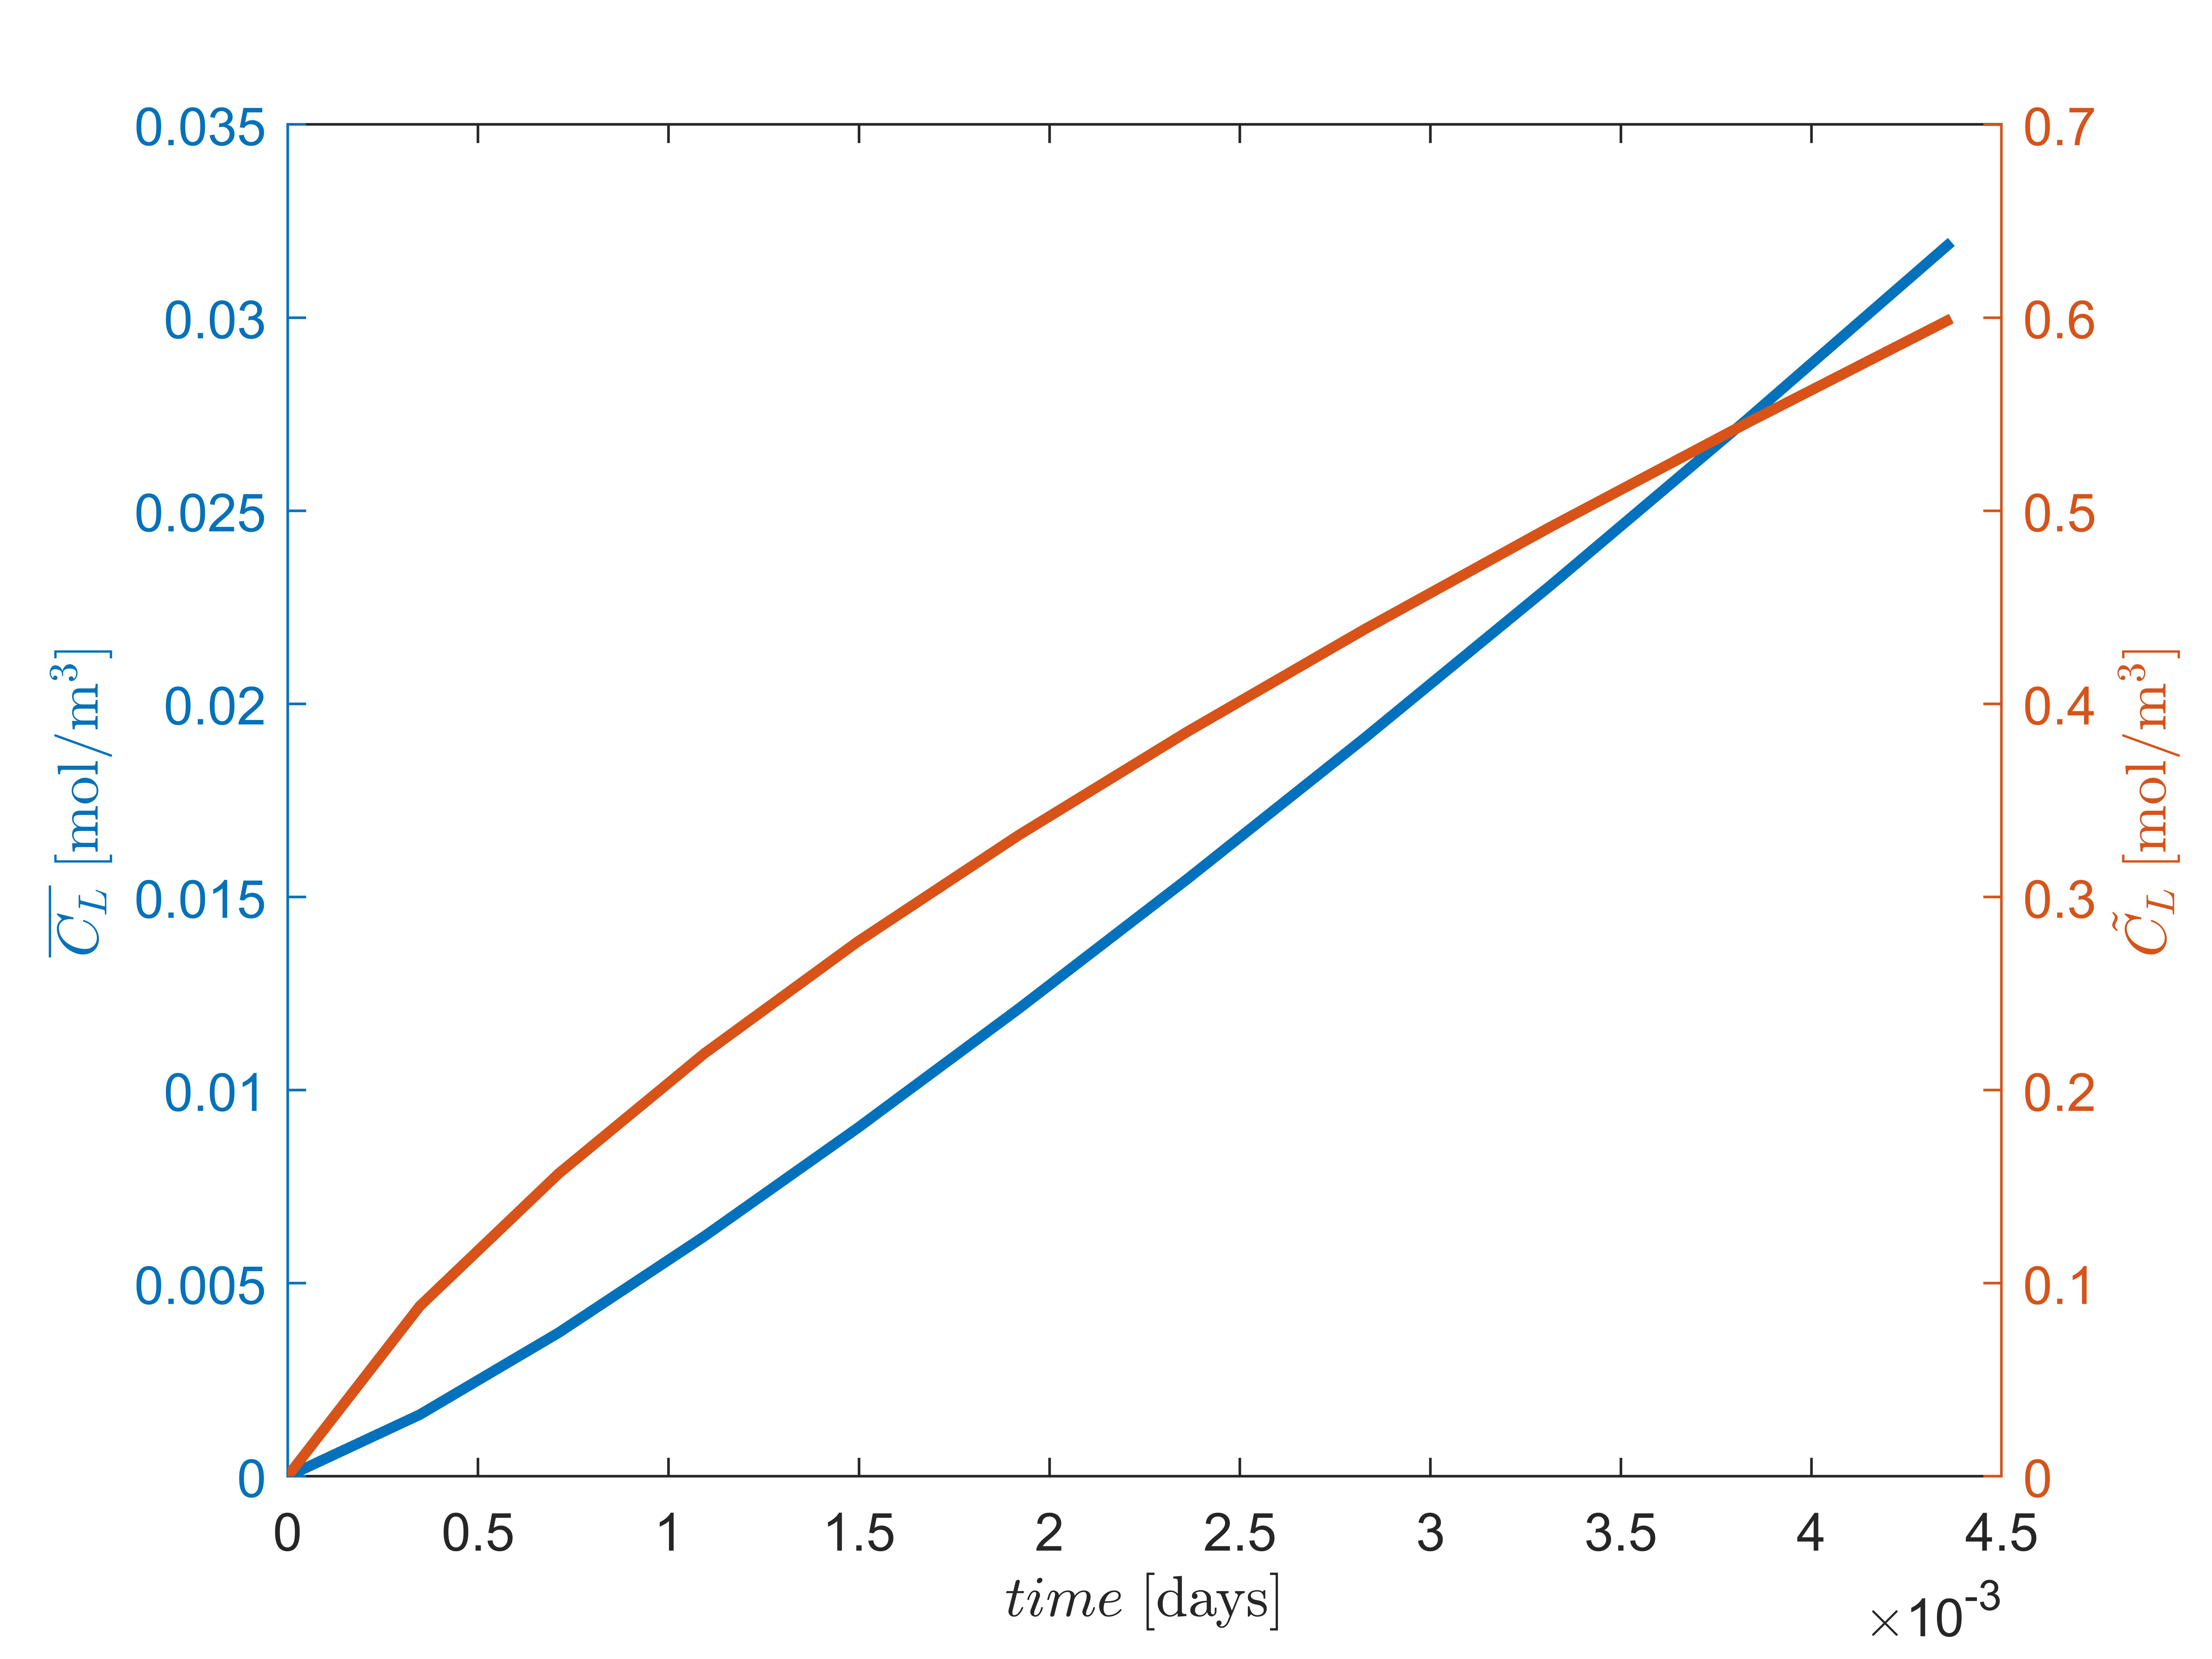
\includegraphics[width=12cm]{../Figures/HydrogenOverTime.jpg}
    \caption{Example of temporal data plotted during the post-processing procedure.}
    \label{fig:example_timedep}
\end{figure}
\begin{figure}
    \centering
    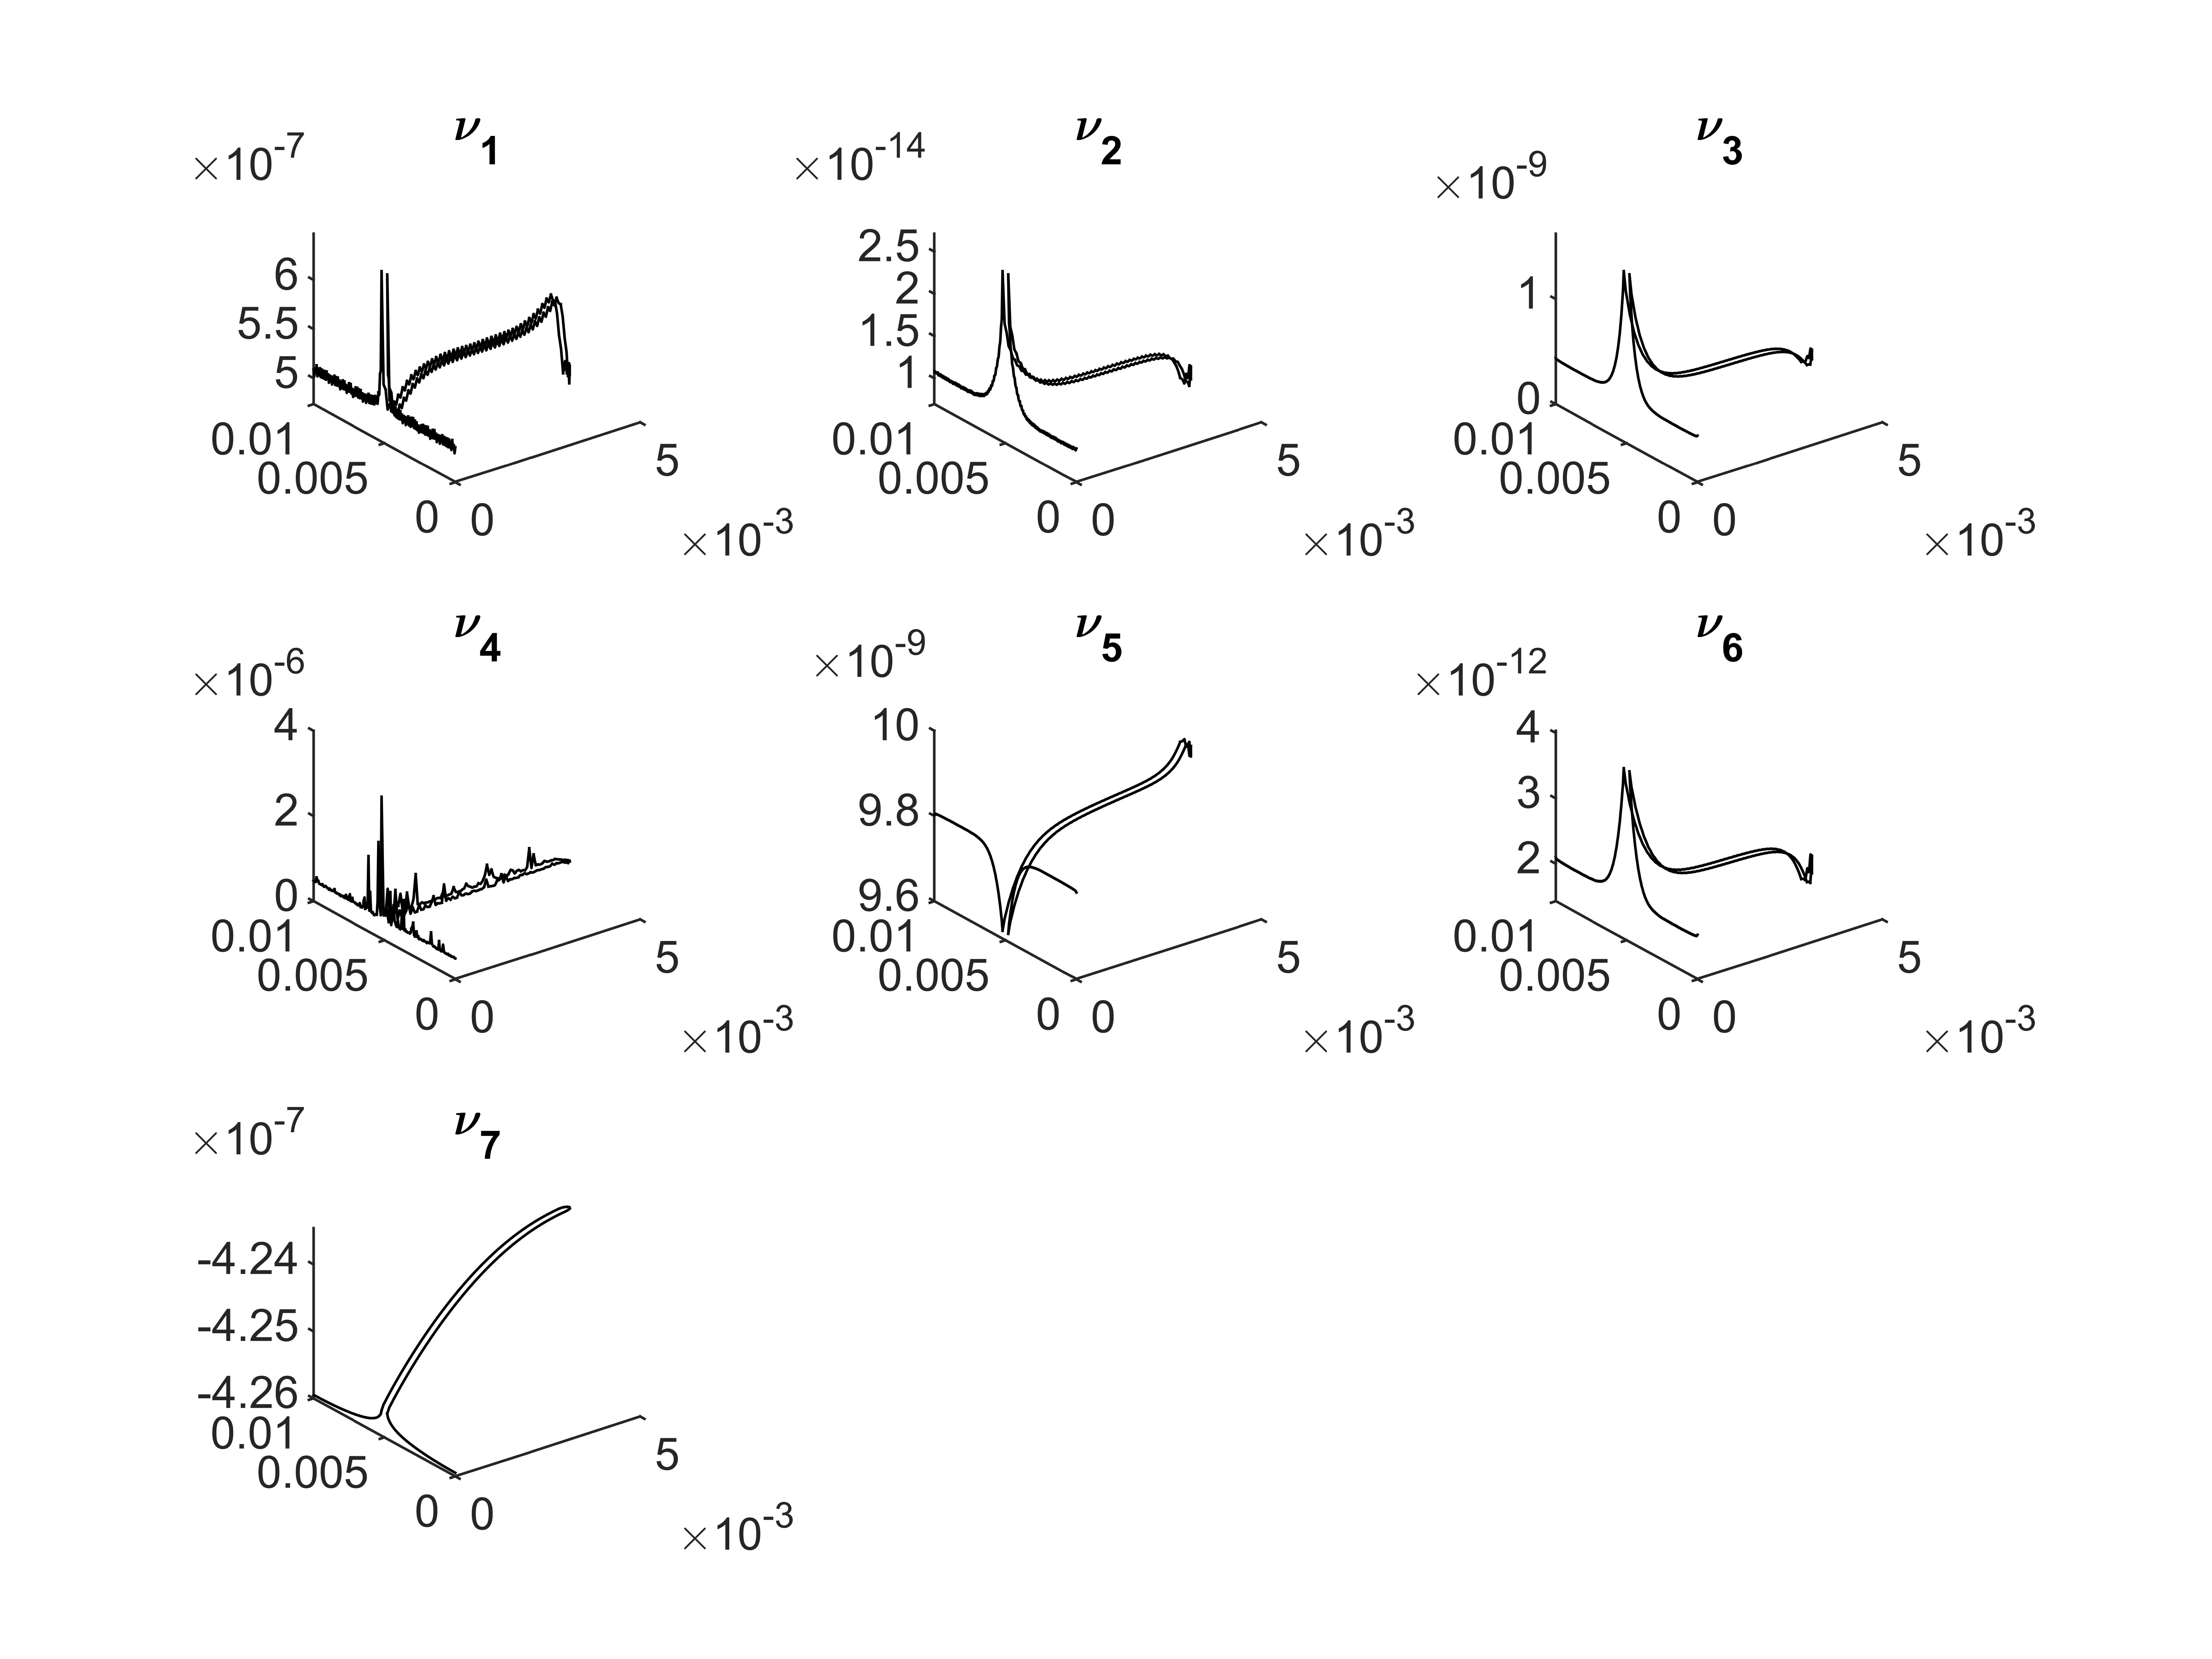
\includegraphics[width=12cm]{../Figures/ReactionRates.jpg}
    \caption{Example of reaction rates plotted during the post-processing procedure.}
    \label{fig:example_rates}
\end{figure}
\begin{figure}
    \centering
    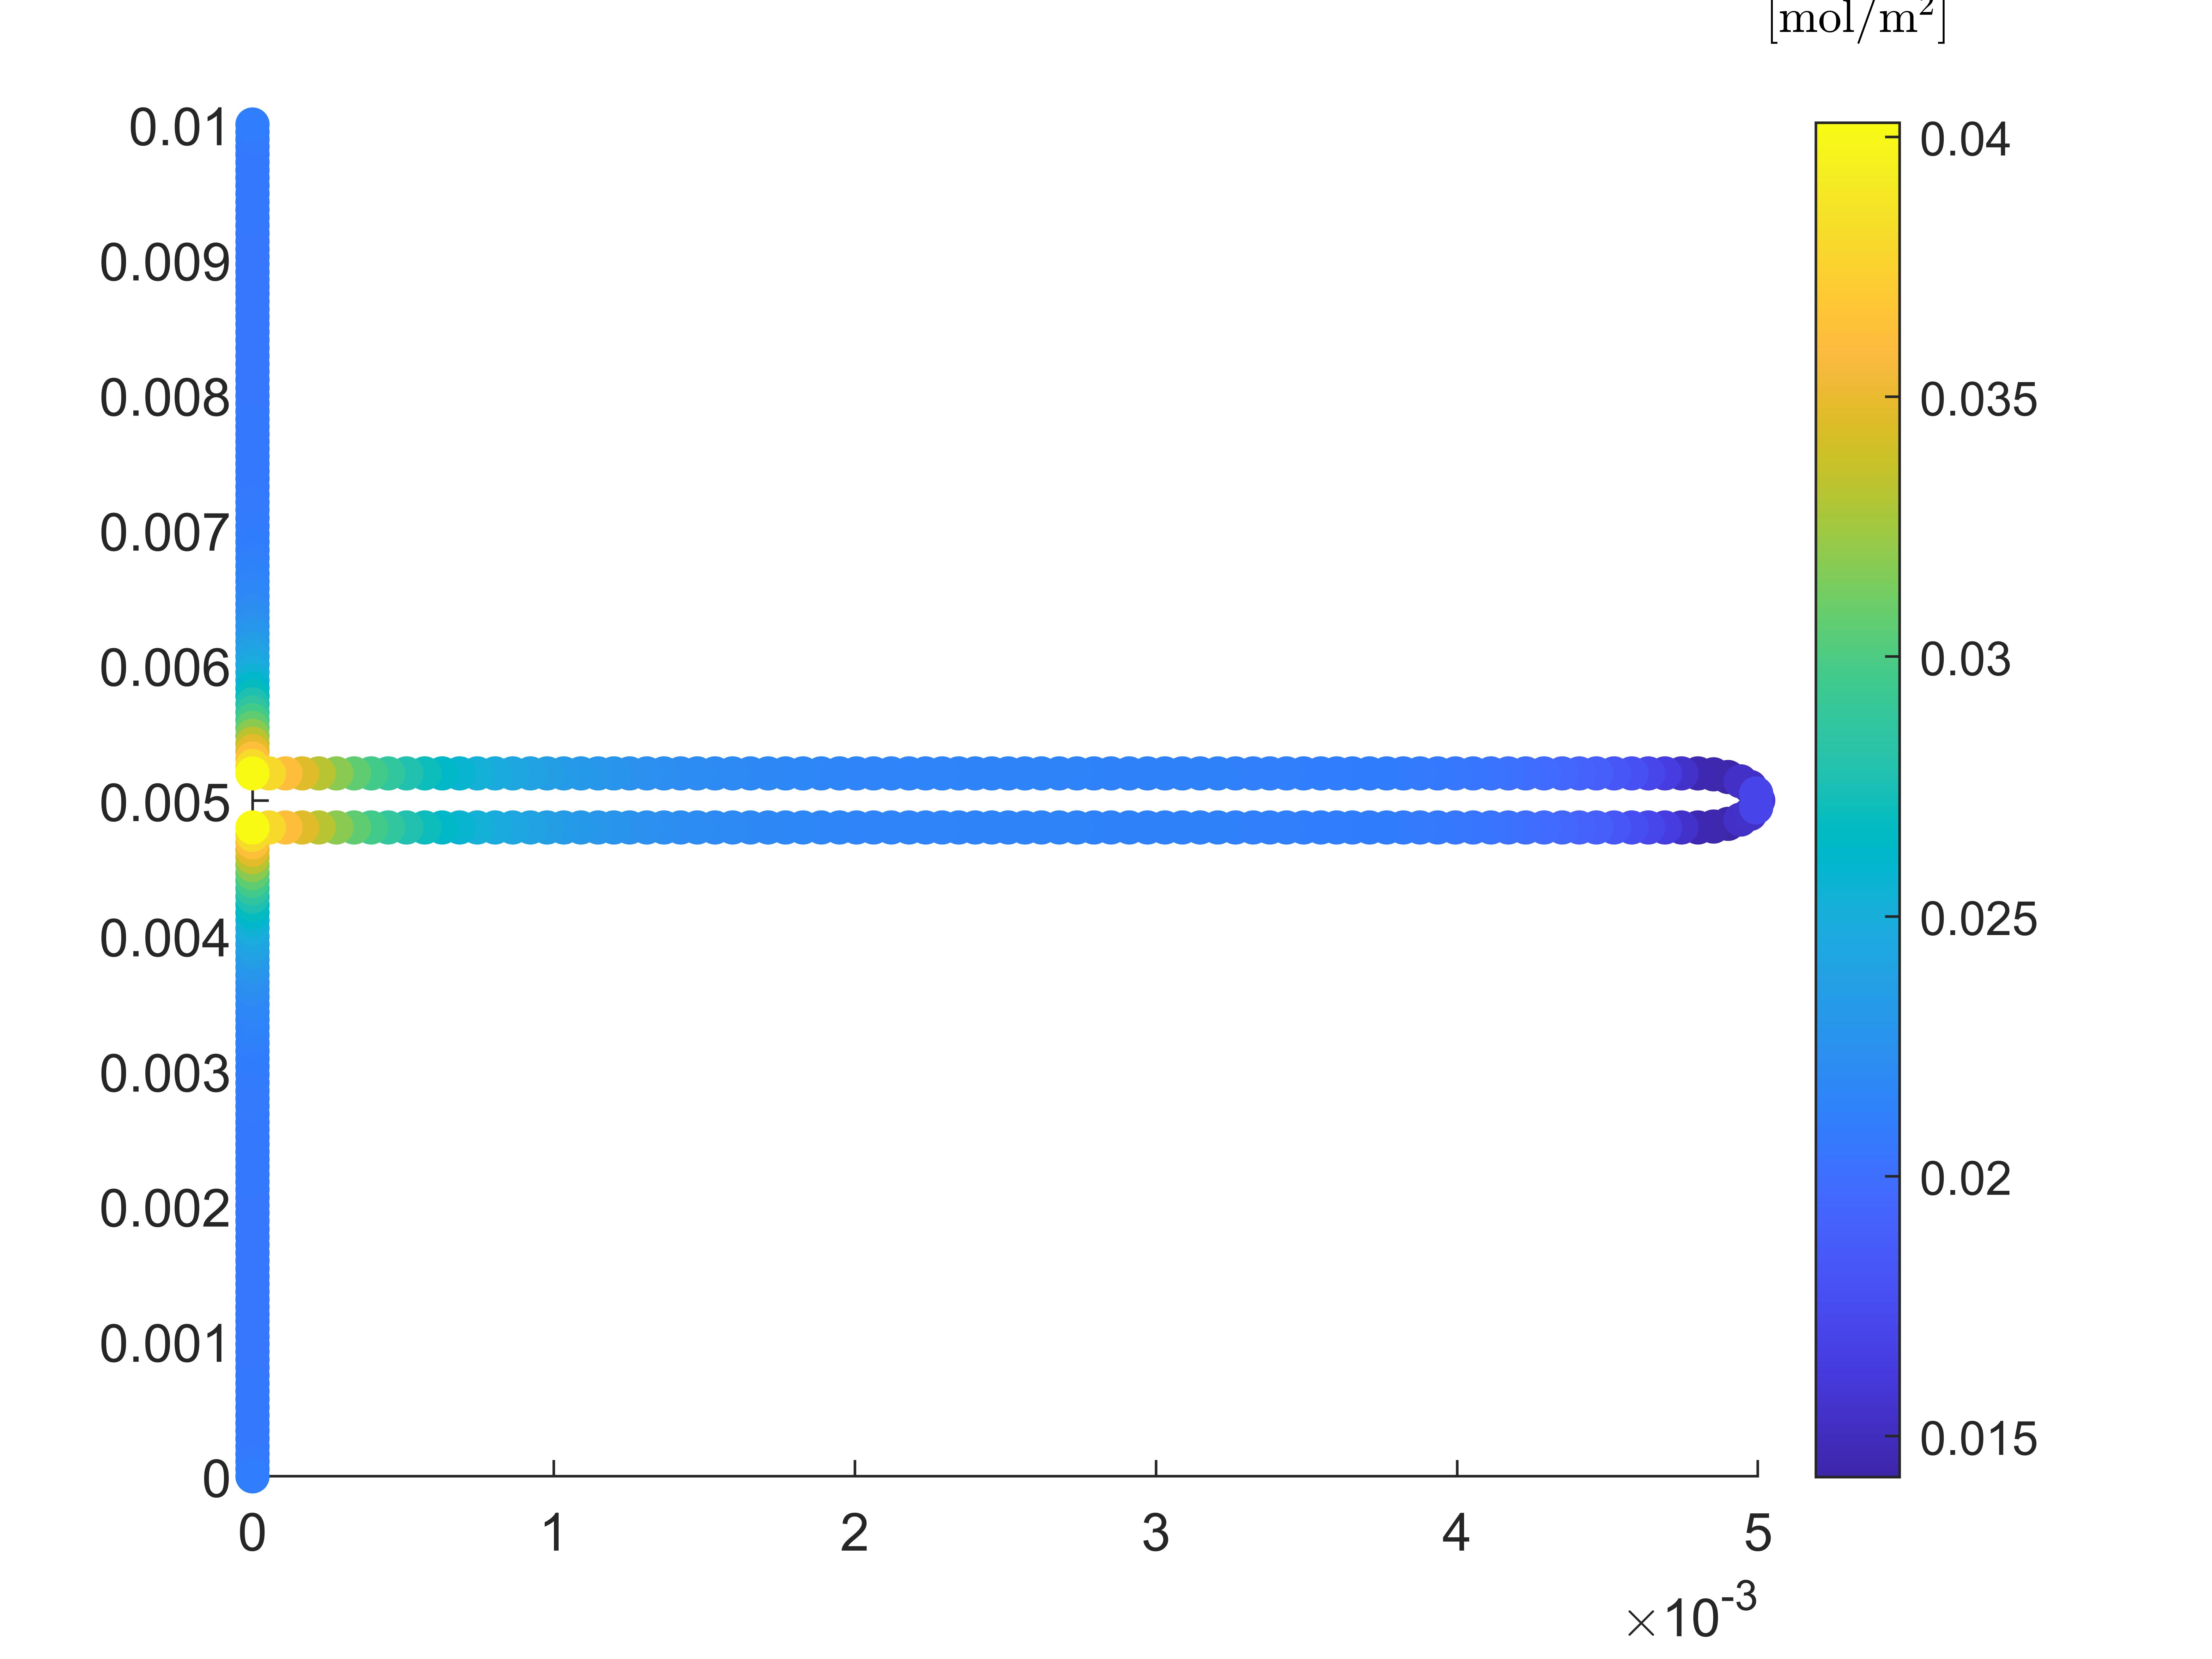
\includegraphics[width=12cm]{../Figures/SurfaceCoverage.jpg}
    \caption{Example of surface coverage plotted during the post-processing procedure.}
    \label{fig:example_coverage}
\end{figure}

Within the simulation code, data files are written at regular intervals. These files can be used for post-processing of the data, and additionally allow for simulations to be resumed from the point when the file was saved. For post-processing, an example is provided within PostProcessing.m, specifically plotting temporal data for the interstitial lattice hydrogen concentration:
\lstinputlisting[firstnumber=12,firstline=12,lastline=26,style=mystyle,title=PostProcessing.m]{../PostProcessing.m}
where the vector tvec contains the time (in seconds) at the end of each time step, the vector CL{\_}vec the volume-averaged hydrogen concentration (in $\mathrm{mol}/\mathrm{m}^3$), and the vector Cmax{\_}vec the maximum hydrogen concentration (also in $\mathrm{mol}/\mathrm{m}^3$). This results in the figure shown in \cref{fig:example_timedep}.

Next, the nodal values of the interstitial lattice hydrogen concentration and pH are plotted as a surface, through the functions:
\lstinputlisting[firstnumber=34,firstline=34,lastline=34,style=mystyle]{../PostProcessing.m}
\lstinputlisting[firstnumber=44,firstline=44,lastline=44,style=mystyle]{../PostProcessing.m}
 with more formatting performed by surrounding functions. This results in \cref{fig:example_surf}. This figure shows the pH at the metal surface increasing due to the hydrogen being adsorbed onto the metal surface. Further into the electrolyte, the metal ions react to produce hydrogen as by-product, reducing the pH. 
 
Reaction rates can be visualised through:
\lstinputlisting[firstnumber=75,firstline=75,lastline=77,style=mystyle]{../PostProcessing.m}
, resulting in \cref{fig:example_rates}. One thing to note is that this plots the reaction rates based on the \textit{integration point} values. As such, small oscillations within these rates are not detrimental for the numerical scheme. The presence of non-physical oscillations can be more directly judges through, for instance, the surface hydrogen coverage, produced by:
\lstinputlisting[firstnumber=80,firstline=80,lastline=85,style=mystyle]{../PostProcessing.m}
 and shown in \cref{fig:example_coverage}, indicating the state of the surface is oscillation-free.

\end{document}
